%%%%%%%%%%%%%%%%%%%%%%%%%%%%%%%%%%%%%%%%%
% Beamer Presentation
% LaTeX Template
% Version 1.0 (10/11/12)
%
% This template has been downloaded from:
% http://www.LaTeXTemplates.com
%
% License:
% CC BY-NC-SA 3.0 (http://creativecommons.org/licenses/by-nc-sa/3.0/)
%
%%%%%%%%%%%%%%%%%%%%%%%%%%%%%%%%%%%%%%%%%

%----------------------------------------------------------------------------------------
%	PACKAGES AND THEMES
%----------------------------------------------------------------------------------------

\documentclass[14pt,handout]{beamer}
%%\documentclass[14pt]{beamer}

\mode<presentation> {

% The Beamer class slide themes
\usetheme{Madrid} %i was using this one

% Beamer class color themes

%\usecolortheme{albatross}

%\setbeamertemplate{footline} % To remove the footer line in all slides uncomment this line
%\setbeamertemplate{footline}[page number] % To replace the footer line in all slides with a simple slide count uncomment this line

%\setbeamertemplate{navigation symbols}{} % To remove the navigation symbols from the bottom of all slides uncomment this line
}

\usepackage{graphicx} % Allows including images
\usepackage{booktabs} % Allows the use of \toprule, \midrule and \bottomrule in tables
\usepackage{hyperref}
\usepackage{helvet}
\usepackage[T1]{fontenc}
\usepackage{textcomp}

%----------------------------------------------------------------------------------------
%	TITLE PAGE
%----------------------------------------------------------------------------------------

\title[Probability and Models]{Statistical Probability and Models} % The short title appears at the bottom of every slide, the full title is only on the title page

\author{C. Ryan Campbell} % Your name
\institute[Duke] % Your institution as it will appear on the bottom of every slide, may be shorthand to save space
{
Duke University \\ % Your institution for the title page
\medskip
\textit{c.ryan.campbell@duke.edu} % Your email address
}
\date{30 Nov 2017} % Date, can be changed to a custom date

\begin{document}

\begin{frame}
\titlepage % Print the title page as the first slide
\end{frame}

%------------------------------------------------
\begin{frame}
\frametitle{Project Update}
\begin{itemize}
	\item<+-> Tuesday - Group AlanAustinRaymond \& ChrisJenniferNayib
	\item<+-> Thursday - Everyone Else
	\item<+-> Present what you have, should be more polished than the rough draft
	\item<+-> 20 minutes per group presentation
	\item<+-> 5min intro, 5min per member
\end{itemize}
\end{frame}

%------------------------------------------------
\begin{frame}
\frametitle{Rough Guidelines}
\begin{itemize}
	\item<+-> Intro group's dataset, \underline{everyone} in your group should participate - 5 mins
	\item<+-> Dicuss your question and results - 5 mins
	\item[]<+-> Suggested order:
	\item<+-> Question/Hypothesis - what did you ask and what did you expect
	\item<+-> Methods - how you asked this question?
	\item<+-> Results - statistical results and plots
	\item<+-> Conclusion - was your hypothesis correct?
	\item<+-> Future Directions/Improvements - what could be done or changed?
\end{itemize}
\end{frame}

\begin{frame}
\frametitle{Overview} % Table of contents slide, comment this block out to remove it
\tableofcontents % Throughout your presentation, if you choose to use \section{} and \subsection{} commands, these will automatically be printed on this slide as an overview of your presentation
\end{frame}

%----------------------------------------------------------------------------------------
%	PRESENTATION SLIDES
%----------------------------------------------------------------------------------------

%------------------------------------------------
\begin{frame}
\frametitle{This Week's Goals}
\begin{itemize}
	\item<+-> Understand p-values \& adjustments
	\item<+-> Learn about Maximum Likelihood
	\item<+-> Learn about Bayes Theorem \& Bayesian Probability
\end{itemize}
\end{frame}

%------------------------------------------------
\section{Probability}
%------------------------------------------------

%------------------------------------------------
\begin{frame}
\frametitle{Probability}
\begin{itemize}
	\item<+-> ``Odds'' that some event occurs
	\item<+-> Bounded from 0 to 1
	\item<+-> Usually expressed as a fraction or percent
	\item<+-> Often using the notation: Pr(event) or P(event)
\end{itemize}
\end{frame}

%------------------------------------------------
\subsection{And versus Or}
%------------------------------------------------

%------------------------------------------------
\begin{frame}
\frametitle{Or}
\begin{itemize}
	\item<+-> Probabilities of multiple events can be combined
	\item<+-> ``Or'' condition
	\item<+-> Probability either thing happens: A or B
	\item<+-> when A and B are independent and mutually exclusive:
	\item<+-> Pr(A or B) = Pr(A) + Pr(B)
\end{itemize}
\end{frame}

%------------------------------------------------
\begin{frame}
\frametitle{Or}
\begin{itemize}
	\item<+-> Probabilities of multiple events can be combined
	\item<+-> ``Or'' condition
	\item<+-> when A and B are independent and \underline{not exclusive}:
	\item<+-> Pr(A or B) = Pr(A) + Pr(B) - Pr(A \& B)
\end{itemize}
\end{frame}

%------------------------------------------------
\begin{frame}
\frametitle{And}
\begin{itemize}
	\item<+-> Probabilities of multiple events both occuring can be combined
	\item<+-> ``And'' condition
	\item<+-> Probability both things happen, A \& B
	\item<+-> When A \& B are independent:
	\item<+-> Pr(A \& B) = Pr(A) * Pr(B)
	\item<+-> ``And'' is commutative:
	\item<+-> Pr(B \& A) = Pr(A \& B)
\end{itemize}
\end{frame}

%------------------------------------------------
\begin{frame}
\frametitle{Conditional Probabilities}
\begin{itemize}
	\item<+-> Probabilities of event A \underline{given} event B
	\item<+-> Probability of A if we know B has occured
	\item<+-> When B happens, how likely is it that A happens
	\item<+-> Numerator = Pr(A \& B)
	\item<+-> Denominator = Pr(B)
	\item<+->[] \underline{Pr(A \& B)}
	\item<+->[] Pr(B)
\end{itemize}
\end{frame}

%------------------------------------------------
\section{Models}
%------------------------------------------------

%------------------------------------------------
\begin{frame}
\frametitle{Models}
\begin{itemize}
	\item<+-> What are models?
	\item<+-> Take in parameters, predict data
	\item<+-> If a die is fair, how many times in 10 rolls should we see a 2?
	\item<+-> BIO EXAMPLE
\end{itemize}
\end{frame}

%------------------------------------------------
\begin{frame}
\frametitle{Models}
\begin{itemize}
	\item<+-> What is an example of a model?
	\item<+-> Mathematical equations that predict experimental results
	\item<+-> Dice are weighted equally, each side should have a 1/6 chance of coming up
	\item<+-> BIO EXAMPLE
\end{itemize}
\end{frame}

%------------------------------------------------
\begin{frame}
\frametitle{Models}
\begin{itemize}
	\item<+-> Why are models useful?
	\item<+-> Allow us to predict results, test those predictions, and put mathematical estimates to natural processes
	\item<+-> Dice example - good for teaching, winning at craps
	\item<+-> BIO EXAMPLE - 
\end{itemize}
\end{frame}

%------------------------------------------------
\begin{frame}
\frametitle{Parameter Estimation}
\begin{itemize}
	\item<+-> Maximum Likelihood
	\item<+-> Bayesian Estimation
\end{itemize}
\end{frame}


%------------------------------------------------
\subsection{Maximum Likelihood}
%------------------------------------------------

%------------------------------------------------
\begin{frame}
\frametitle{Maximum Likelihood}
\begin{itemize}
	\item<+-> Parameters for which the data are most likely are correct
	\item<+-> Vary the parameters and check how likely the data are
	\item<+-> ``Plug \& Chug''
\end{itemize}
\end{frame}

%------------------------------------------------
\begin{frame}
\frametitle{Conditional Probabilities}
\begin{itemize}
	\item<+-> Probabilities of data \underline{given} parameters/model
	\item<+-> With these parameters, how likely is this data?
	\item<+-> Numerator = Pr(params \& data)
	\item<+-> Denominator = Pr(data)
	\item<+->[] \underline{Pr(params \& data)}
	\item<+->[] Pr(data)
\end{itemize}
\end{frame}

%------------------------------------------------
\begin{frame}
\frametitle{Maximum Likelihood}
\begin{itemize}
	\item<+-> Likelihoods aren't meaningful alone
	\item<+-> Only used relative to other likelihoods from the same model
	\item<+-> Greatest likelihood is accepted as the parameter's value
\end{itemize}
\end{frame}

%------------------------------------------------
\begin{frame}
\frametitle{Maximum Likelihood: Toy Example}
\begin{itemize}
	\item<+-> I flipped a coin 10 times
	\item<+-> 6 Heads \& 4 Tails
	\item<+-> Model - Binary probability distribution \& Pr(head) = 1 - Pr(tails)
	\item<+-> What is the true probability of it landing heads?
\end{itemize}
\end{frame}

%------------------------------------------------
\begin{frame}
\frametitle{Maximum Likelihood: Toy Example}
\begin{itemize}
	\item<+-> Binary Probabilty Distribution
	\begin{center}
	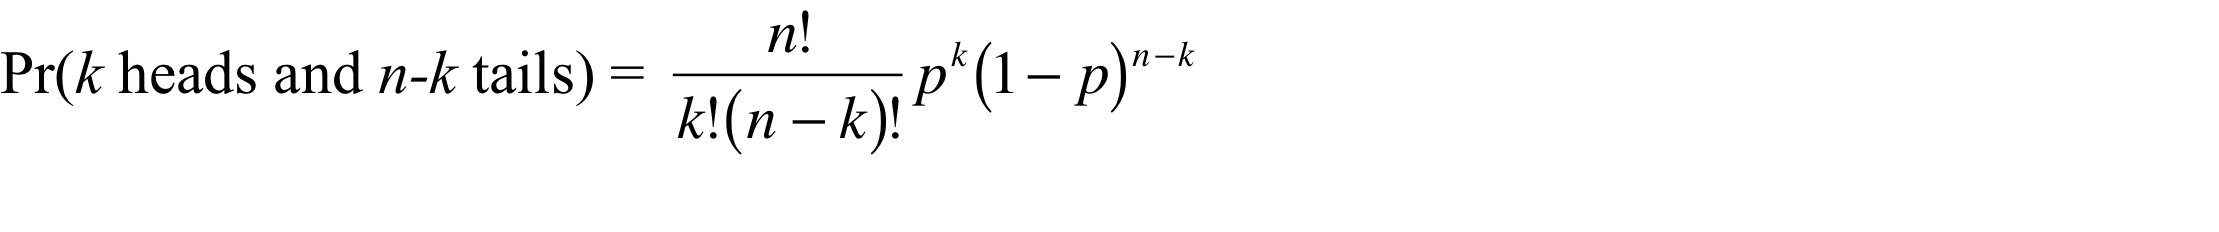
\includegraphics[width=1.5\textwidth]{images_20171130_binProb.png}
	\end{center}
	\item<+-> Which are data and which are parameters (of n, k \& p)?
\end{itemize}
\end{frame}

%------------------------------------------------
\begin{frame}
\frametitle{Maximum Likelihood: Toy Example}
\begin{itemize}
	\item<+-> What is the probability of seeing this data (6H 4T):
	\item<+-> If the coin is 50-50?
	\item<+-> If the coin is 75-25?
\end{itemize}
\end{frame}

%------------------------------------------------
\begin{frame}
\frametitle{Maximum Likelihood: Toy Example}
\begin{itemize}
	\ttfamily
	\footnotesize
	\begin{block}{}
		\item[]  n <- 10
		\item[]  k <- 6
		\item[]  p <- .5
		\item[]  
		\item[]  prD <- (factorial(n) / (factorial(k) * factorial(n - k))) * p\^{}k * (1 - p)\^{}(n - k)
	\end{block}
	\normalsize
	\sffamily
	\item<+-> What is the probability of the coin being 50-50?
	\item<+-> What about 75-25?
	\item<+-> Can you plot the results of many values of p?
	\item<+->[] hint: use \texttt{seq()}
\end{itemize}
\end{frame}

%------------------------------------------------
\begin{frame}
\frametitle{Maximum Likelihood: Toy Example}
\begin{itemize}
	\ttfamily
	\footnotesize
	\begin{block}{}
		\item[]  p <- seq(0,1,.01)
		\item[]  prD <- (factorial(n) / (factorial(k) * factorial(n - k))) * p\^{}k * (1 - p)\^{}(n - k)
		\item[]  plot(p,prD)
	\end{block}
	\begin{center}
	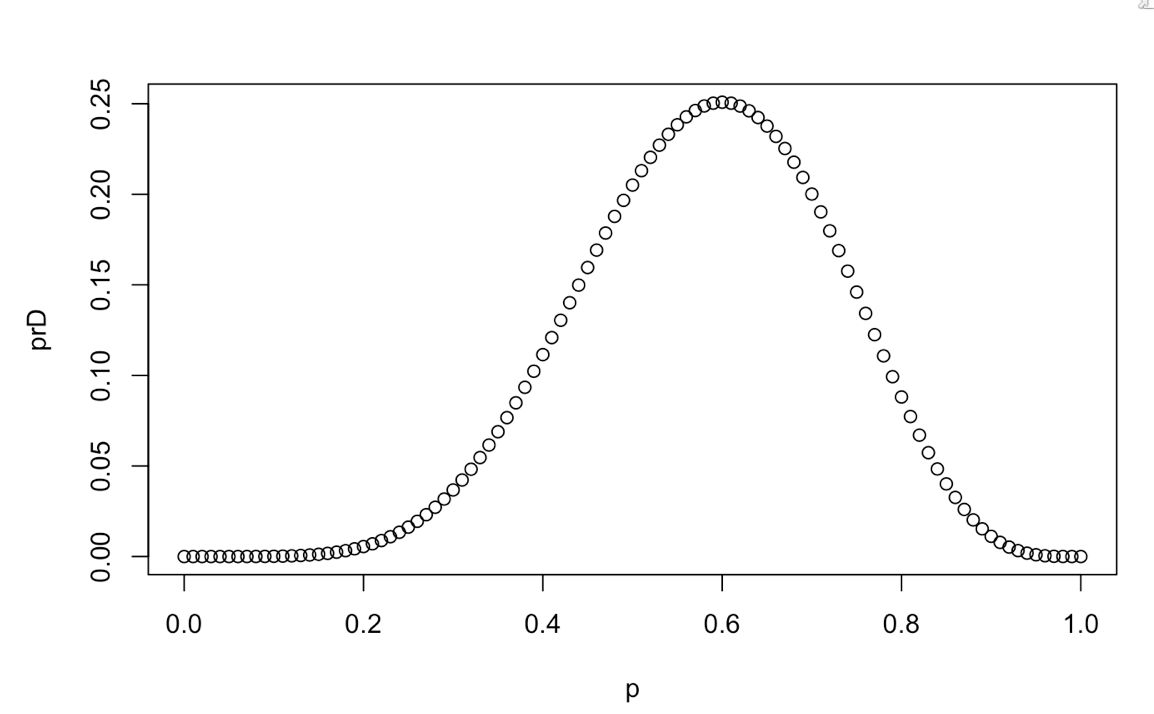
\includegraphics[width=0.75\textwidth]{images_20171130_MLresults.png}
	\end{center}
\end{itemize}
\end{frame}

%------------------------------------------------
\begin{frame}
\frametitle{Maximum Likelihood}
\begin{itemize}
	\item<+-> Strictly following the Maximum Likelihood to estimate the parameter:
	\item<+-> What is the true probability of the coin landing on heads?
	\item<+-> Does this seem accurate?
	\item<+-> Why is this a misleading example?
\end{itemize}
\end{frame}

%------------------------------------------------
\begin{frame}
\frametitle{Maximum Likelihood: Bio Example}
\begin{itemize}
	\item<+-> Normally used for complicated parameters and datasets
	\item<+-> Estimating mutation rates or branch lengths on a phylogeny
	\item<+-> What models would be useful for RNAseq?
\end{itemize}
\end{frame}

%------------------------------------------------
\begin{frame}
\frametitle{Maximum Likelihood: Bio Example}
\begin{itemize}
	\item<+-> What models would be useful for RNAseq?
	\item<+-> Inferring isoform expression levels:
	\item[]<+-> (given a proprotion of reads mapping to exons, how many of each isoform are present)
	\item<+-> Gene pathway interactions:
	\item[]<+-> (given a set of expression across the genes in a gene pathway, are they being activated together?)
\end{itemize}
\end{frame}

%------------------------------------------------
\subsection{Bayes Rule}
%------------------------------------------------

%------------------------------------------------
\begin{frame}
\frametitle{Conditional Probabilities}
\begin{itemize}
	\item<+-> Probabilities of data \underline{given} parameters/model
	\item<+-> With these parameters, how likely is this data?
	\item<+-> Numerator = Pr(params \& data)
	\item<+-> Denominator = Pr(data)
	\item<+->[] \underline{Pr(params \& data)}
	\item<+->[] Pr(data)
\end{itemize}
\end{frame}

%------------------------------------------------
\begin{frame}
\frametitle{Deriving Bayes Rule}
	\begin{center}
	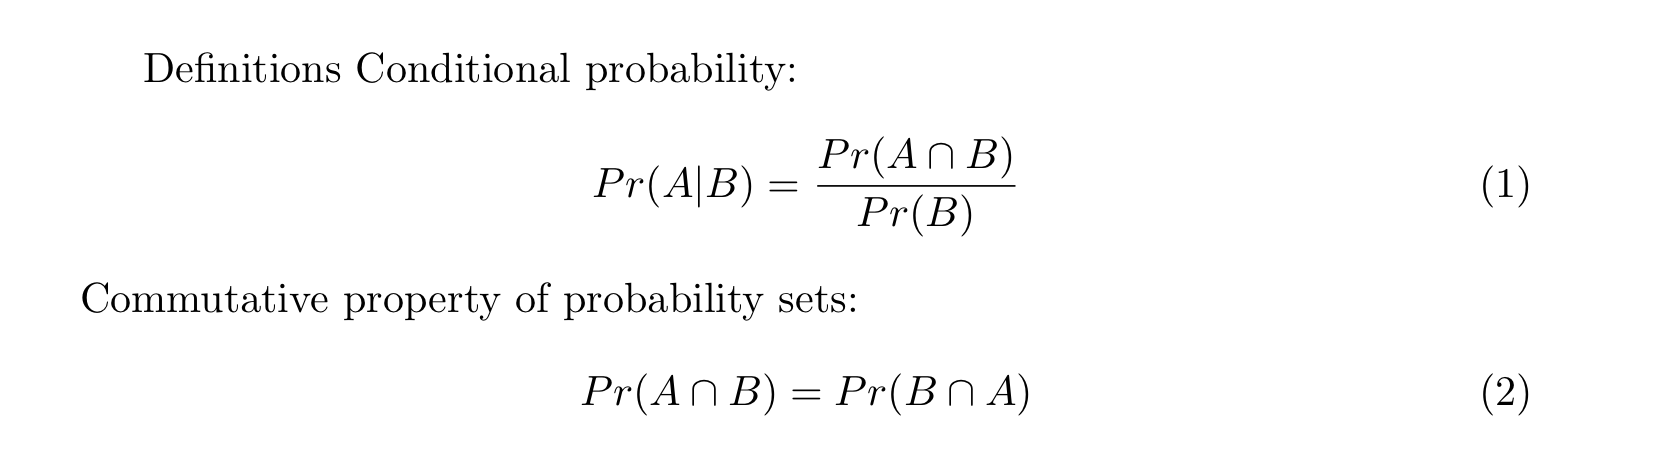
\includegraphics[width=0.75\textwidth]{images_20171130_bayes_1and2.png}
	\end{center}
	\begin{center}
	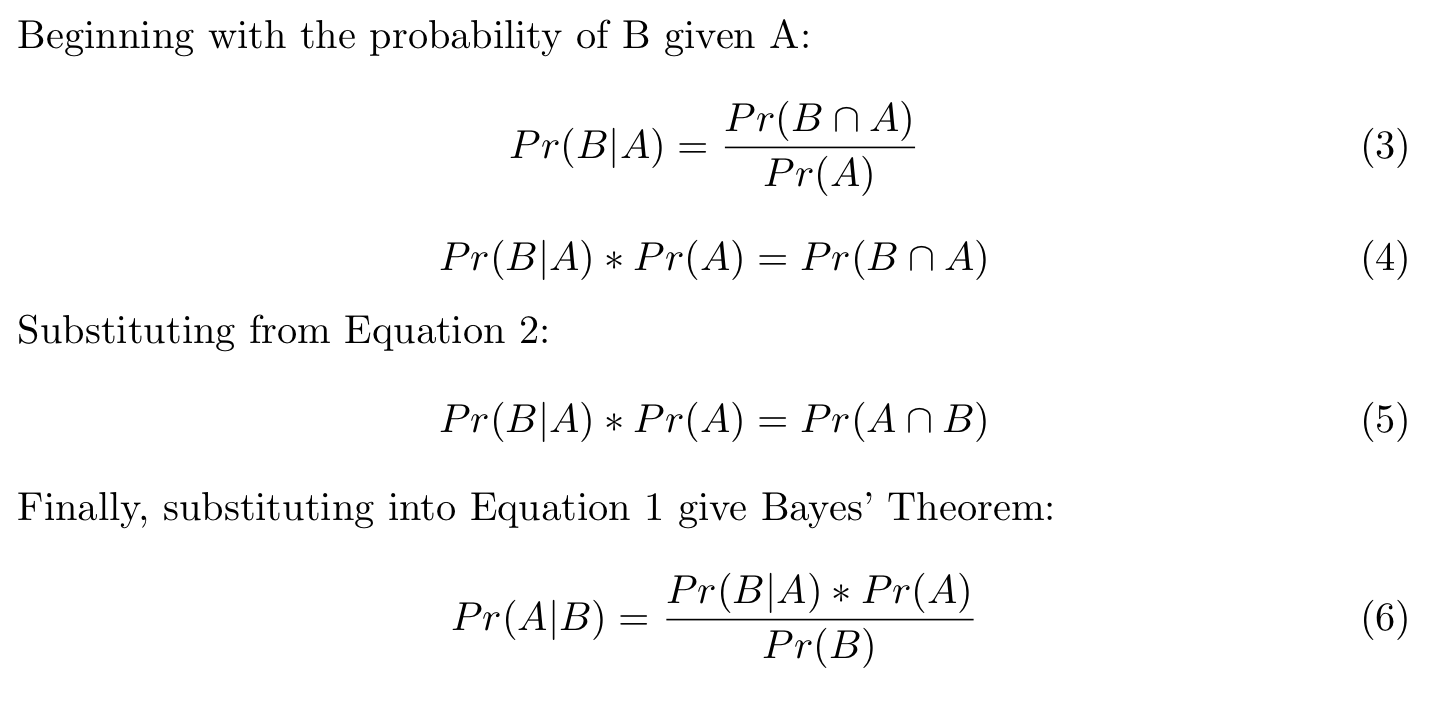
\includegraphics[width=0.85\textwidth]{images_20171130_bayes.png}
	\end{center}
\end{frame}

%------------------------------------------------
\begin{frame}
\frametitle{Bayes Rule}
\begin{itemize}
\item[] 
	\begin{center}
	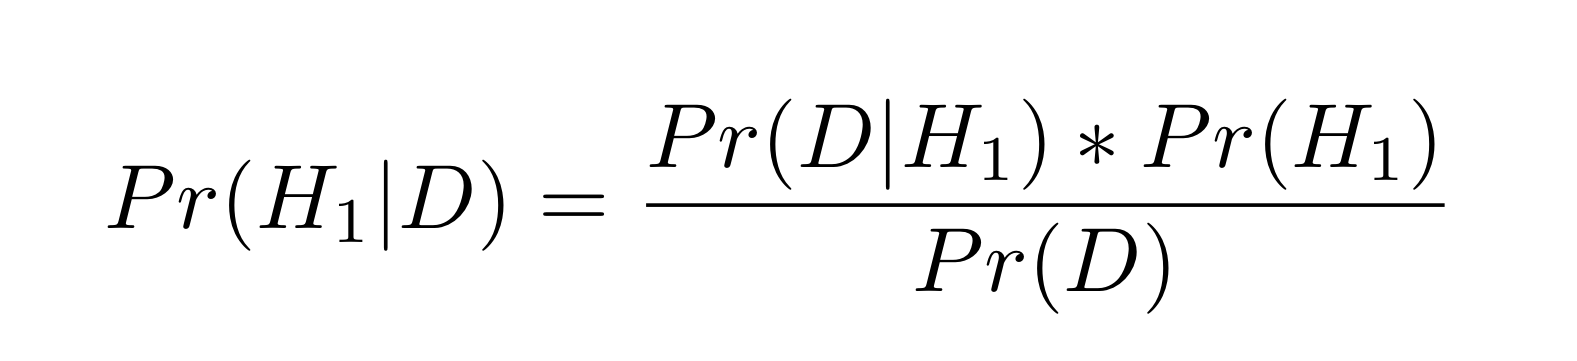
\includegraphics[width=0.75\textwidth]{images_20171130_bayes_final.png}
	\end{center}
	\item<+-> Likelihood
	\item<+-> Prior
	\item<+-> Posterior
\end{itemize}
\end{frame}

%------------------------------------------------
\begin{frame}
\frametitle{Bayes Rule}
\begin{itemize}
	\item<+-> Likelihood - probability of the data given the hypothesis
	\item<+-> Prior - probability of the hypothesis
	\item<+-> Posterior - probability of the hypothesis given the data (what we want!)
\end{itemize}
\end{frame}

%------------------------------------------------
\begin{frame}
\frametitle{Bayes Rule}
\begin{itemize}
\item[] 
	\begin{center}
	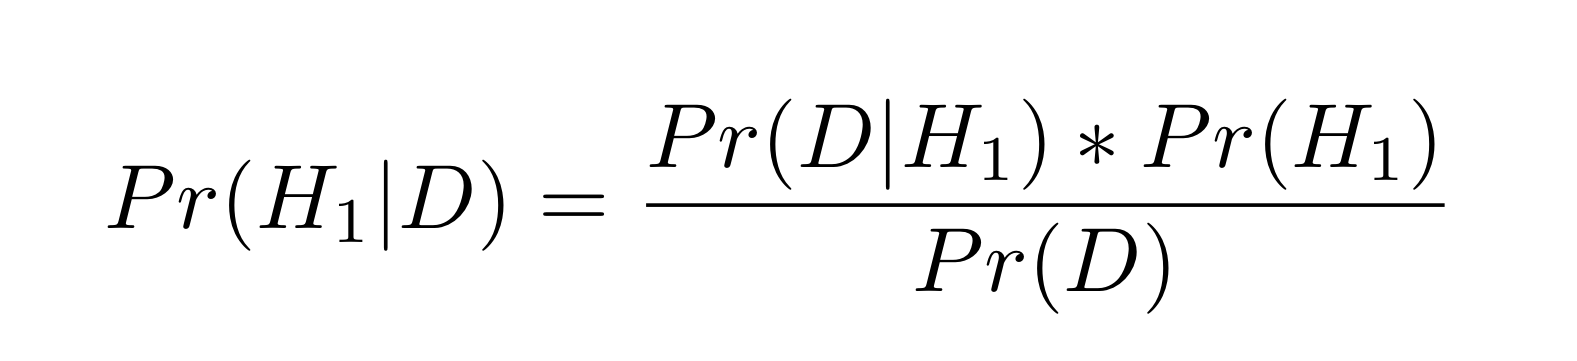
\includegraphics[width=0.75\textwidth]{images_20171130_bayes_final.png}
	\end{center}
	\item<+-> Likelihood
	\item<+-> Prior
	\item<+-> Posterior
\end{itemize}
\end{frame}

%------------------------------------------------
\section{ML versus Bayes Rule: An Example}
%------------------------------------------------

%------------------------------------------------
\begin{frame}
\frametitle{Bayesian: Toy Example}
\begin{itemize}
	\item<+-> I flipped a coin 10 times
	\item<+-> 6 Heads \& 4 Tails
	\item<+-> Model - Binary probability distribution \& Pr(head) = 1 - Pr(tails)
	\item<+-> What is the true probability of it landing heads?
\end{itemize}
\end{frame}

%------------------------------------------------
\begin{frame}
\frametitle{Bayesian: Toy Example}
\begin{itemize}
	\item<+-> Binary Probabilty Distribution
	\begin{center}
	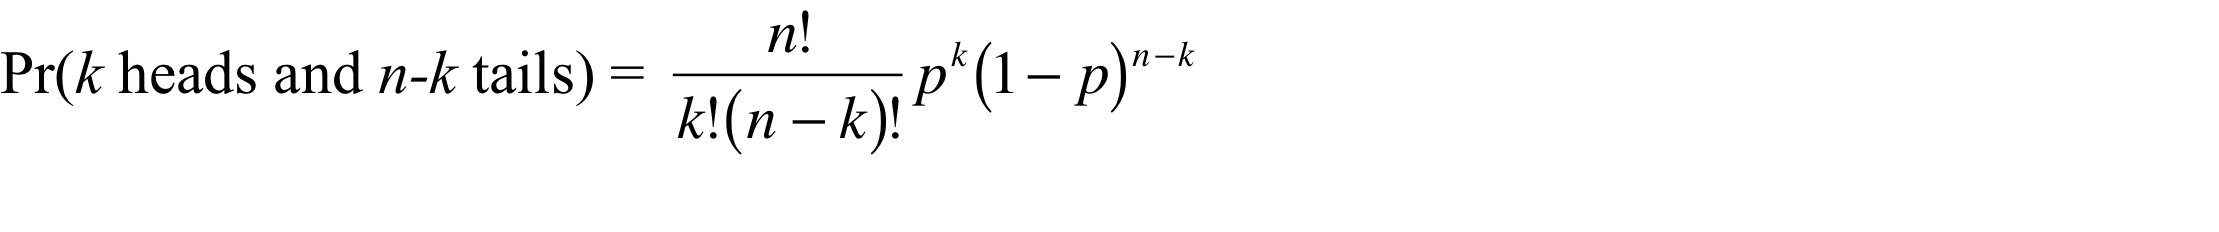
\includegraphics[width=1.5\textwidth]{images_20171130_binProb.png}
	\end{center}
	\item<+-> Which are data and which are parameters (of n, k \& p)?
\end{itemize}
\end{frame}

%------------------------------------------------
\begin{frame}
\frametitle{Bayesian: Toy Example}
\begin{itemize}
	\item<+-> What is the prior probability of the parameters?
	\item<+-> The coin is 50-50?
	\item<+-> The coin is 75-25?
\end{itemize}
\end{frame}

%need to add prior

%------------------------------------------------
\begin{frame}
\frametitle{Bayesian: Toy Example}
\begin{itemize}
	\ttfamily
	\footnotesize
	\begin{block}{}
		\item[]  n <- 10
		\item[]  k <- 6
		\item[]  p <- .5
		\item[]  
		\item[]  prD <- (factorial(n) / (factorial(k) * factorial(n - k))) * p\^{}k * (1 - p)\^{}(n - k)
	\end{block}
	\normalsize
	\sffamily
	\item<+-> How do we add the prior in?
\end{itemize}
\end{frame}

%------------------------------------------------
\begin{frame}
\frametitle{Bayesian: Toy Example}
\begin{itemize}
	\item<+-> Prior Distribution
	\begin{center}
	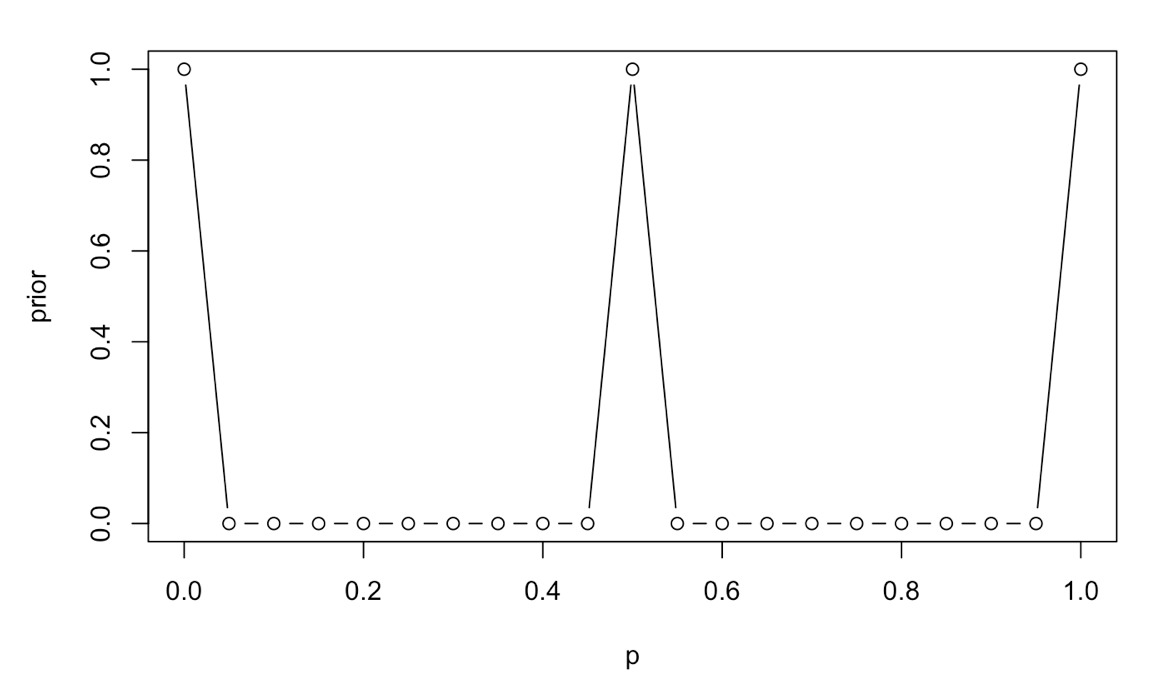
\includegraphics[width=0.8\textwidth]{images_20171130_prior.png}
	\end{center}
\end{itemize}
\end{frame}

%------------------------------------------------
\begin{frame}
\frametitle{Bayesian: Toy Example}
\begin{itemize}
	\item<+-> Posterior Distribution
	\begin{center}
	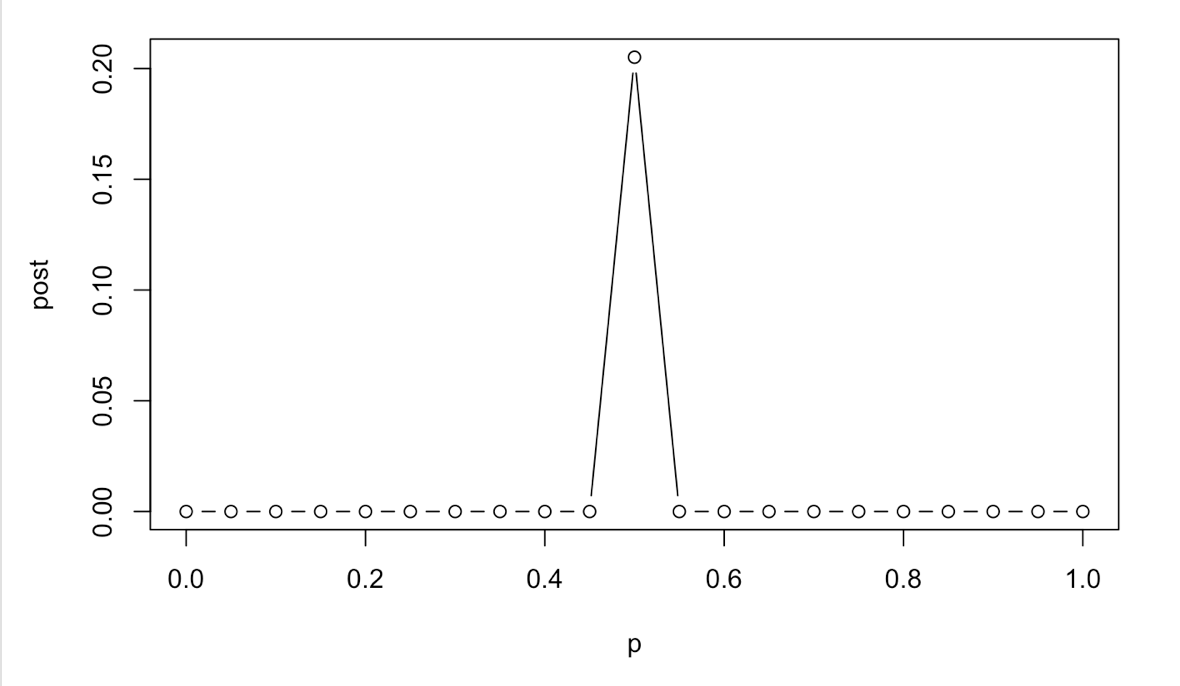
\includegraphics[width=0.8\textwidth]{images_20171130_posterior.png}
	\end{center}
\end{itemize}
\end{frame}

%------------------------------------------------
\begin{frame}
\frametitle{Bayesian: Toy Example}
\begin{itemize}
\item[] 
	\begin{center}
	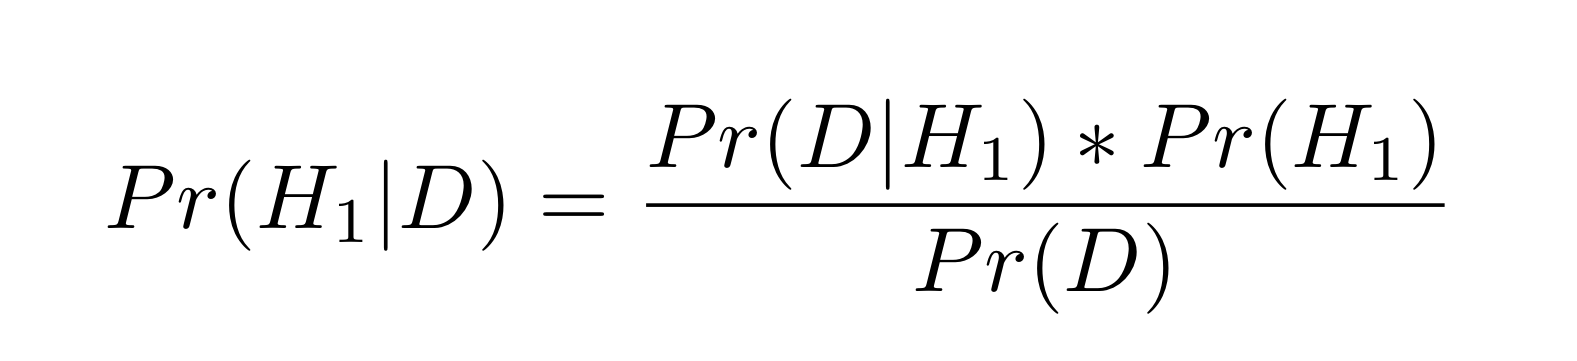
\includegraphics[width=0.75\textwidth]{images_20171130_bayes_final.png}
	\end{center}
	\item<+-> Likelihood
	\item<+-> Prior
	\item<+-> Posterior
\end{itemize}
\end{frame}

%------------------------------------------------
\begin{frame}
\frametitle{Bayesian Parameter Estimation}
\begin{itemize}
	\item<+-> Following the Bayesian Estimation:
	\item<+-> What is the true probability of the coin landing on heads?
	\item<+-> Does this seem accurate?
\end{itemize}
\end{frame}

%------------------------------------------------
\begin{frame}
\frametitle{Bayes vs. ML}
\begin{itemize}
	\item<+-> What is the main difference?
	\item<+-> What problems might come along with a prior?
	\item<+-> What are biologically relevant problems that this method solves?
\end{itemize}
\end{frame}

%------------------------------------------------
\begin{frame}
\frametitle{More XKCD}
	\begin{center}
	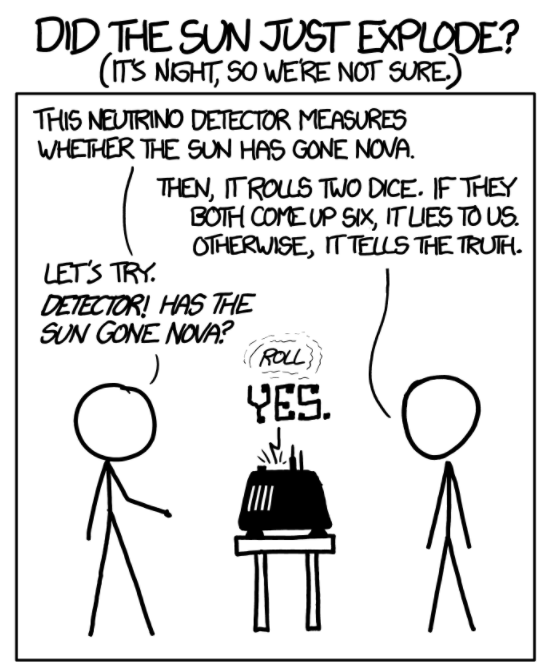
\includegraphics[width=0.55\textwidth]{images_20171130_xkcd1.png}
	\end{center}
\end{frame}

%------------------------------------------------
\begin{frame}
\frametitle{More XKCD}
	\begin{center}
	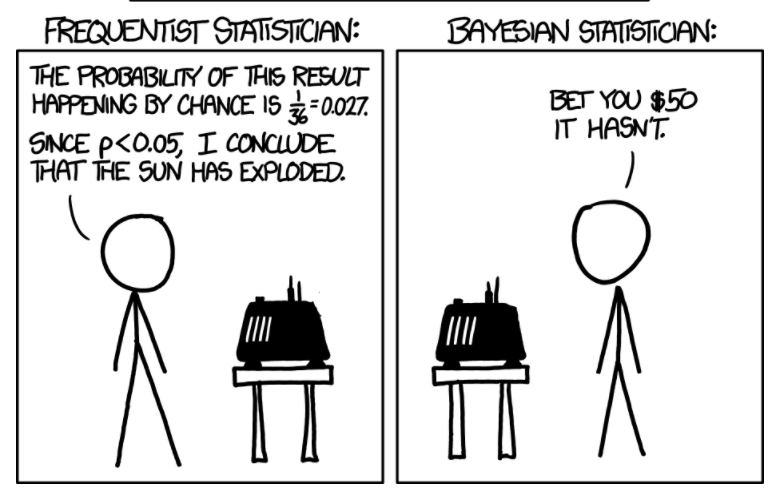
\includegraphics[width=0.95\textwidth]{images_20171130_xkcd2.png}
	\end{center}
\end{frame}

%------------------------------------------------
\begin{frame}
\Huge{\centerline{The End}}
\end{frame}

%----------------------------------------------------------------------------------------

\end{document} 